% 2.2.QandA.tex
%	Last update: 2020/02/13 F.Kanehori
%newpage
\subsection{Q\&A}
\label{subsec:QandA}
\parindent=0pt

前項\KQuote{\ref{subsec:PreparationForApp} ビルドの準備} に従って作成した
アプリケーションに関するQ\&A集です。
以下\SprLib の Base プロジェクトを例にとって説明しますが、
他のプロジェクト(Collision, Foundation, $\cdots$)についても同様です。

\Important{%
	unix上で\SprLib とアプリケーションの並行開発を行なうことはないと思われますので、
	ここではWindows上でVisual Studioを使う場合について説明します。}
\bigskip

%-------------------------------------------------------------------------------
\thinrule{\linewidth}
\bf{プログラムの実行時に“リソースファイルが見つからない”というエラーが起きる}

\medskip
プログラムは作業ディレクトリ\BldDir 下に作成されます。
プログラムが相対パス指定でリソースを参照している場合には、
CMakeLists{} があるディレクトリ(\Path{C:/Develop/Application})から
プログラムを起動してください

%-------------------------------------------------------------------------------
\thinrule{\linewidth}
\bf{ソリューションファイルに新しいターゲットがある}

\tt{ALL\_BUILD}
\begin{narrow}
	これはCMakeが自動的に作成するターゲットで、
	\tt{make all}に相当するものとされています。
	ただしVisual Studio上では\tt{ALL\_BUILD}の依存関係の設定が不正確で、
	このターゲットをビルドしても正しい結果は得られないようです。
	\bf{このターゲットは無視してください}
\end{narrow}

\tt{sync}
\begin{narrow}
	これはプロジェクトファイルの整合性を保つために作られたターゲットで、
	他のターゲットをビルドすることにより自動的にこのターゲットが最初に実行されます。
	\bf{このターゲットに対して何らかのアクションを起こす必要はありません。}
	\KQuote{\ref{subsec:Problems:ProjectFileIntegration}
	プロジェクトファイルの整合性} 参照。
\end{narrow}

%-------------------------------------------------------------------------------
\thinrule{\linewidth}
\bf{ソリューションまたはプロジェクトが環境外で変更された旨のメッセージが出る}

\medskip
これはアプリケーション側と\SprLib 側との整合性を保つために
上記の\tt{sync}ターゲットが実行されることで、
ソリューションファイル / プロジェクトファイルが変更されることがあるためです。
すべて\bf{再読み込み}としてください。

\Important{%
	実際には、新しく生成されたプロジェクトファイルを取り込むために、
	ソリューションファイル中のProjectGuidを書き直すことがあるためです。\\
	なお、「再読み込み」を指定するとVisual Studioの出力ウィンドウに表示されている
	メッセージがすべてクリアされてしまいます。
	これを防ぐには、一旦「無視」を指定し、
	その後にソリューションを開き直せば同じ結果が得られます。}

%-------------------------------------------------------------------------------
\thinrule{\linewidth}
\bf{ディレクトリが作成できないエラーが発生する}

\medskip
\SprLib をビルドすると、ソースツリー上に\\
\hspace{10pt}\Path{C:/Springhead/core/src/Base/\it{x64}/\it{15.0}/Base.dir} \\
というディレクトリが作成されます(\it{x64}, \it{15.0}の部分は環境により異なります)。

アプリケーションの\cmake をした後で上記のディレクトリを削除すると、
以降のビルドで

\hspace{20pt}``エラー MSB3191 ディレクトリ "Base.dir/Debug/" を作成できません''

などというエラーが発生します。

\bf{この問題を解消するためには、
アプリケーション側または\SprLib 側で 再度\cmake を実行する必要があります。}

また、\SprLib 側で\cmake (configure)を実行していないと 
上記のディレクトリが作成されていないため、同じエラーが発生します。
\bf{この場合には、\SprLib 側で\cmake を実行してください。}

%-------------------------------------------------------------------------------
\thinrule{\linewidth}
\bf{ビルドの最適性が崩れる}
\label{subsec:QandA:CrumbleBuildOptimizeation}

\medskip
アプリケーション側で\Path{C:/Develop/Application/build/Base.Base.dir}などを削除すると、
ビルド時にVisual Studioが\BldDir 下に\Path{Base.dir}を自動的に作成してしまうために
ビルドの最適性が崩れてしまいます。

\Important{%
	無駄なビルドが発生するだけで、ビルド自体は正常に行なえます。
	``ビルドの最適性''については\KQuote{\ref{subsubsec:Problems}問題点} を
	参照してください。}

\medskip
\bf{この問題を解消するためには、
アプリケーション側または\SprLib 側で 再度\cmake を実行する必要があります。}

%-------------------------------------------------------------------------------
\thinrule{\linewidth}
\bf{sync configurationでファイルオープンエラーが発生する}

\medskip
\SprLib 側で\Path{\BldDir/Base}下にあるプロジェクトファイル
\Path{Base.vcxproj}を削除すると、
sync ターゲット実行でlink先のファイルが見つからずに

\CmndLine{%
	> 1>sync configuration with C:/Springhead/core/src \\
	> \hspace{10pt}:\\
	> 1>Error : file open error : "Base/Base.vcxproj" \\
	> 1>Traceback (most recent call last): \\
	> \hspace{10pt}:\\
}{command-2-2.eps}{cmake}

のようなエラーが発生します。

\bf{この問題を解消するためには、
\SprLib 側で再度\cmake を実行する 必要があります (アプリケーション側では駄目)。}

%-------------------------------------------------------------------------------
\thinrule{\linewidth}
\bf{2019/9/30 (commit 1d8e5ce) 以前に配布したバージョンをご使用の場合}

\bf{新しい配布ファイルから \CMakeLists{} を再作成すれば、 以下の問題は解消します。}

\medskip
上記以前のバージョンで配布した\QCMakeLists{.*.dist}を元に\QCMakeLists{}を作成して
使用している場合は、 RunSwigでclean/rebuildの対応ができていなかったため、
cleanと同等の機能を実現するためのターゲットRunSwig\_Clean が作成されているはずです。
\bf{上記日付以降の\SprLib をダウンロードし\cmake を実行していただければ、
RunSwigはclean/rebuild 対応となります。}

\Important{%
	RunSwig\_Cleanをビルドすると\\
	\hspace{15pt}\tt{python: can't open file '.../Clean.py': ... No such file ...}\\
	というエラーが起きます。
	実害はありませんがRunSwigのcleanは行なわれません。}

RunSwig\_Clean ターゲットを生成されないようにするには、
\QCMakeLists{}から以下の部分を削除して再\cmake してください。

\begin{narrow}\begin{figure}[h]
    \begin{narrow}[30pt]
	\begin{center}\fbox{%
	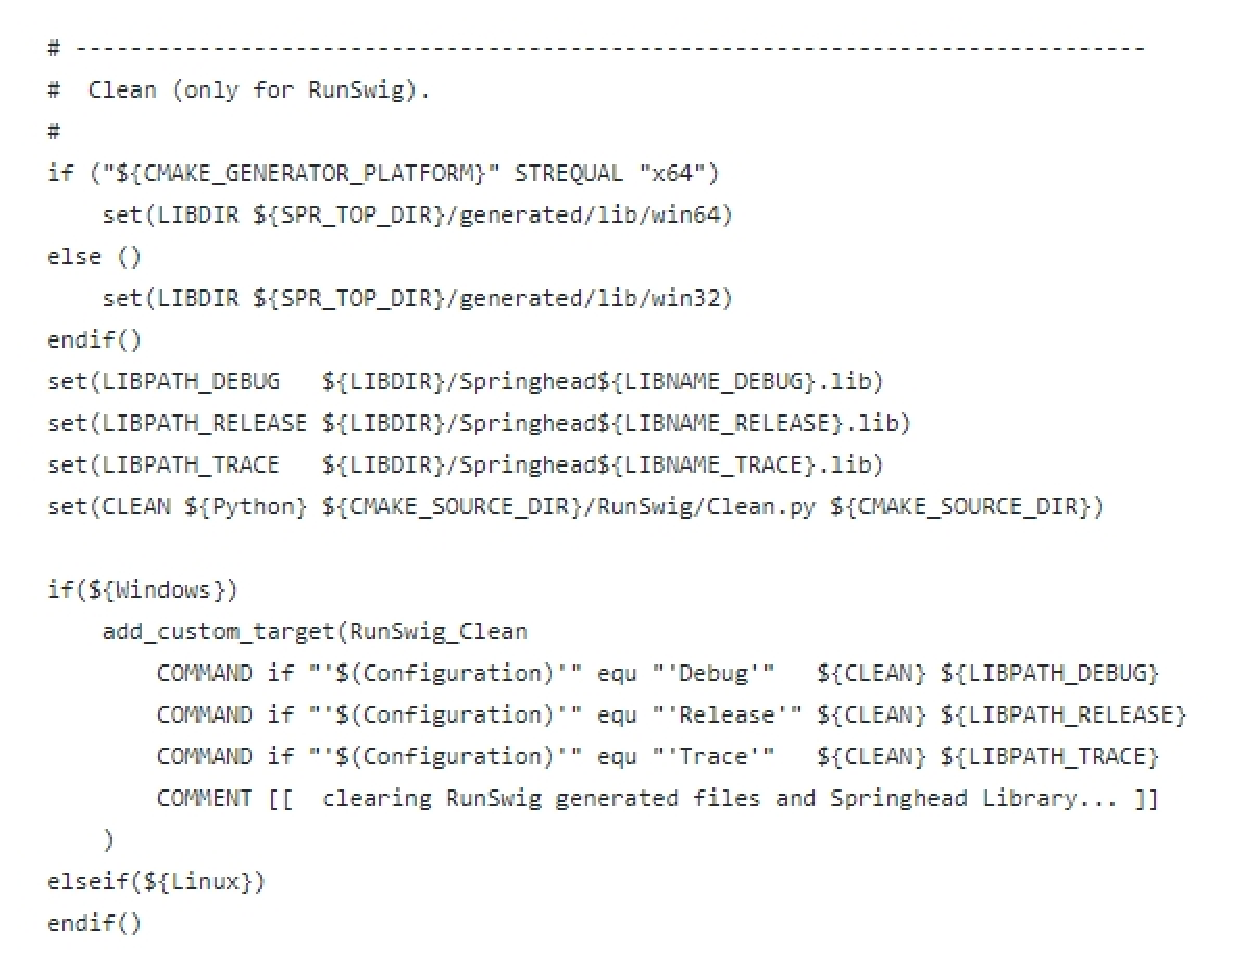
\includegraphics[width=.8\textwidth]{fig/RemoveRunSwigClean.eps}
	}\end{center}
	\label{fig:SpringheadLibraryTree}
    \end{narrow}
\end{figure}\end{narrow}
	
EmbPython\_RunSwig\_Cleanについても同様です。	

% end: 2.2.QandA.tex
